\documentclass{lehramt-informatik}
\usepackage{amsmath}
\usepackage{blkarray}
\usepackage{tikz}
\usetikzlibrary{arrows.meta}

\begin{document}

%%%%%%%%%%%%%%%%%%%%%%%%%%%%%%%%%%%%%%%%%%%%%%%%%%%%%%%%%%%%%%%%%%%%%%%%
% Theorie-Teil
%%%%%%%%%%%%%%%%%%%%%%%%%%%%%%%%%%%%%%%%%%%%%%%%%%%%%%%%%%%%%%%%%%%%%%%%

\chapter{Graphen}

\begin{quellen}
\item \cite[Seite 445-481 (PDF 461-505)]{saake}
\item \cite{wiki:graph}
\end{quellen}

\noindent
Ein Graph ist eine \memph{dynamische Datenstruktur}, die die
\memph{Speicherung beliebig vieler Elemente} erlaubt. Ein Graph besteht
aus \memph{Knoten} und \memph{Kanten}, die die Beziehungen zwischen den
Knoten repräsentieren

\section{Arten von Graphen}

\begin{compactitem}
\item gerichtete / ungerichtete Graphen
\item gewichtete / ungewichtete Graphen
\end{compactitem}

\section{Grad}

\begin{compactitem}
\item Eingangsgrad (Anzahl der eingehenden Kanten)
\item Ausgangsgrad (Anzahl der ausgehenden Kanten)
\item Bei ungerichteten Graphen: Grad
\end{compactitem}

\footcite[Seite 3]{aud:fs:6}

\noindent
Ein Graph ist ein Paar $G=(V, E)$. $V$ bezeichnet die Menge der Knoten
(\memph{vertex}) und $E \subseteq V \times V$ die Menge der Kanten
(\memph{edge}).
%
Eine Kante $(a, b) \in E$ ist im \emph{gerichteten} Graphen eine Kante
von $a$ nach $b$. Im \emph{ungerichteten} Graphen schreiben wir $[a,b]$.
Dabei ist $(a, b) \in E$ und $(b, a) \in E$.
%
Im gerichteten Graphen gibt es analog zu
Listen und Bäumen Vorgänger- und Nachfolgerknoten. Jeder Kante $e \in
E$ kann ein \memph{Kantengewicht} $c(e)$ zugeordnet sein. Kantengewichte
entsprechen den „Kosten“ für die Traversierung dieser Kante. Die
Darstellung von Graphen ist auf unterschiedliche Weise möglich:

\begin{compactitem}
\item graphische Darstellung
\item Mengenschreibweise
\item Adjazenzmatrix
\item Adjazenzlisten
\end{compactitem}
\footcite[Seite 4]{aud:fs:6}

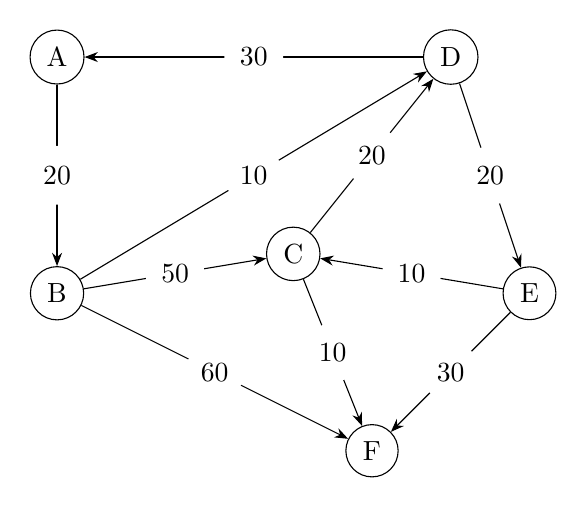
\begin{tikzpicture}
\begin{scope}[every node/.style={circle,draw}]
\node (A) at (0,0) {A};
\node (B) at (0,-3) {B};
\node (C) at (3,-2.5) {C};
\node (D) at (5,0) {D};
\node (E) at (6,-3) {E};
\node (F) at (4,-5) {F};
\end{scope}

\begin{scope}[>={Stealth[black]},
              every node/.style={fill=white,circle},
              every edge/.style={draw=black}]
\path [->] (A) edge node {20} (B);
\path [->] (B) edge node {10} (D);
\path [->] (B) edge node {50} (C);
\path [->] (B) edge node {60} (F);
\path [->] (C) edge node {20} (D);
\path [->] (C) edge node {10} (F);
\path [->] (D) edge node {20} (E);
\path [->] (D) edge node {30} (A);
\path [->] (E) edge node {10} (C);
\path [->] (E) edge node {30} (F);
\end{scope}
\end{tikzpicture}

%-----------------------------------------------------------------------
%
%-----------------------------------------------------------------------

\section{Adjazenz-Matrix}

Eine \textbf{Adjazenzmatrix} (von lat. \emph{adiacere} = bei oder neben
etwas liegen, angrenzen) eines Graphen ist eine Matrix, die speichert,
welche Knoten des Graphen durch eine Kante verbunden sind. Sie besitzt
für \memph{jeden Knoten} eine \memph{Zeile} und eine \memph{Spalte},
woraus sich für $n$ Knoten eine $n \times n$-Matrix ergibt. Ein Eintrag
in der $i$-ten Zeile und $j$-ten Spalte gibt hierbei an, ob eine Kante
von dem $i$-ten zu dem $j$-ten Knoten führt
\footcite{wiki:adjazenzmatrix}. Man geht \memph{von der Zeile zur
Spalte}.

%%
%
%%

\subsection{Die Adjazenzmatrix eines ungerichteten Graphen}

Eine Verbindung (Kante) zwischen zwei Knoten in einem ungerichteten
Graphen ist in beide Richtungen gültig. Überträgt man die Verbindungen
in die Matrix, erhält man eine \memph{symmetrische, an der Diagonalen
gespiegelte Adjazenzmatrix}.

%%
%
%%

\subsection{Die Adjazenzmatrix eines gerichteten Graphen}

Beim gerichteten Graphen sind die Verbindungen zwischen den Knoten
jeweils nur in einer Richtung gültig. Im Graphen erfolgt die Darstellung
der \memph{Richtung mit einem Pfeil}. Für die Adjazenzmatrix haben die
gerichteten Kanten zur Folge, dass \memph{keine Symmetrie mehr} besteht.

%%
%
%%

\subsection{Die Adjazenzmatrix für Graphen mit Kantengewichten}

In gewichteten Graphen haben die Kanten sogenannte Kosten oder Gewichte.
In einer Matrix für gewichtete Graphen werden keine Nullen und Einsen,
sondern die \memph{Werte für das jeweilige Gewicht} der Kante zwischen
den Knoten eingetragen.
\footnote{\url{https://www.bigdata-insider.de/was-ist-eine-adjazenzmatrix-a-845891/}}

\[
\begin{blockarray}{ccccccc}
& A & B & C & D & E & F \\
\begin{block}{c(cccccc)}
A & 0  & 20 & 0  & 0  & 0  & 0  \\
B & 0  & 0  & 50 & 10 & 0  & 60 \\
C & 0  & 0  & 0  & 20 & 0  & 10 \\
D & 30 & 0  & 0  & 0  & 20 & 0  \\
E & 0  & 0  & 10 & 0  & 0  & 30 \\
F & 0  & 0  & 0  & 0  & 0  & 0  \\
\end{block}
\end{blockarray}
\]

%https://tex.stackexchange.com/a/24378
\usetikzlibrary{matrix,arrows,fit}

\tikzset{circarrow/.style={
        *->,
        shorten <=-2pt
    }
}

\begin{tikzpicture}[>=stealth]
\matrix (M) [matrix of nodes,%
   column sep=-\pgflinewidth,%
   row sep=1mm,%
   nodes in empty cells,
   nodes={draw, fill=gray!20,%
     minimum width=.5cm, outer sep=0pt,%
     minimum height=.7cm, anchor=center},
   column 1/.style={nodes={minimum height=.8cm}}]%
{
  &[2mm] 2 & &[2mm] 5 & /  \\
 & 1 & & 5 & &[2mm] 3 & &[2mm] 4 & / \\
 & 2 & & 5 & & 3 & /\\
};

\foreach \i in {1,2,3}{
 \path (M-\i-1) [late options={label=left:\i}];
 \draw[->] (M-\i-1)--(M-\i-2.west);
 \draw[->] (M-\i-3.center)--(M-\i-4.west);
}

\draw[->] (M-2-5.center)--(M-2-6.west);
\draw[->] (M-2-7.center)--(M-2-8.west);
\draw[->] (M-3-5.center)--(M-3-6.west);
\end{tikzpicture}

\literatur
\end{document}
